\subsection{The Two-Level Awareness Structure: Self and Community}
\label{subsec:11-4-two-level-structure}

%%%%%%%%%%%%%%%%%%%%%%%%%%%%%%%%%%%%%%%%%%%%%%%%%%%%%%%%%%%%%%%%%%%%%%%%%%%%%%%
% SECTION 11.4: The Two-Level Structure
% Module: BCM2_05_AWX_7240
% Content: Self vs. Community × INU/KNU/IDN = 6 Components
%%%%%%%%%%%%%%%%%%%%%%%%%%%%%%%%%%%%%%%%%%%%%%%%%%%%%%%%%%%%%%%%%%%%%%%%%%%%%%%

From the content definition, awareness encompasses effects on \emph{both}
one's own utility \emph{and} the utility of a relevant community. This
creates a two-level, six-component awareness structure.

%------------------------------------------------------------------------------
\subsubsection{The Complete Awareness Matrix}
%------------------------------------------------------------------------------

\begin{equation}
\boxed{
\mathbf{A} = \begin{pmatrix}
A^{self}_{INU} & A^{self}_{KNU} & A^{self}_{IDN} \\
A^{comm}_{INU} & A^{comm}_{KNU} & A^{comm}_{IDN}
\end{pmatrix}
}
\label{eq:awareness-matrix}
\end{equation}

\begin{table}[htbp]
\centering
\caption{The Complete Awareness Matrix: Six Components}
\label{tab:awareness-matrix-complete}
\renewcommand{\arraystretch}{1.5}
\begin{tabular}{@{}l|ccc@{}}
\toprule
& \textbf{INU} & \textbf{KNU} & \textbf{IDN} \\
\midrule
\textbf{Own utility} & $A^{self}_{INU}$ & $A^{self}_{KNU}$ & $A^{self}_{IDN}$ \\
& Effects on MY welfare & Effects on OUR group & Effects on WHO I AM \\
\midrule
\textbf{Community utility} & $A^{comm}_{INU}$ & $A^{comm}_{KNU}$ & $A^{comm}_{IDN}$ \\
& Effects on THEIR welfare & Effects on THEIR groups & Effects on WHO THEY ARE \\
\bottomrule
\end{tabular}
\end{table}

%------------------------------------------------------------------------------
\subsubsection{The Six Awareness Questions}
%------------------------------------------------------------------------------

Each component corresponds to a distinct question the decision-maker may
(or may not) be asking at the Moment of Truth:

\begin{table}[htbp]
\centering
\caption{The Six Awareness Questions}
\label{tab:six-questions}
\renewcommand{\arraystretch}{1.4}
\begin{tabular}{@{}llll@{}}
\toprule
\textbf{Component} & \textbf{Question} & \textbf{Focus} & \textbf{Default $A$} \\
\midrule
$A^{self}_{INU}$ & What does this do for ME? & Personal gains/pains & HIGH \\
$A^{self}_{KNU}$ & What does this do for US? & Group welfare I belong to & MEDIUM \\
$A^{self}_{IDN}$ & What does this say about WHO I AM? & Identity confirm/threat & LOW-MEDIUM \\
$A^{comm}_{INU}$ & What does this do for THEM? & Others' personal welfare & LOW \\
$A^{comm}_{KNU}$ & What does this do for THEIR groups? & Others' collective welfare & VERY LOW \\
$A^{comm}_{IDN}$ & What does this do to WHO THEY ARE? & Others' identity & VERY LOW \\
\bottomrule
\end{tabular}
\end{table}

%------------------------------------------------------------------------------
\subsubsection{The Awareness Gradient}
%------------------------------------------------------------------------------

There is a systematic gradient in default awareness levels:

\begin{equation}
\boxed{A^{self}_{INU} > A^{self}_{KNU} > A^{self}_{IDN} > A^{comm}_{INU} > A^{comm}_{KNU} > A^{comm}_{IDN}}
\label{eq:awareness-gradient}
\end{equation}

\begin{figure}[htbp]
\centering
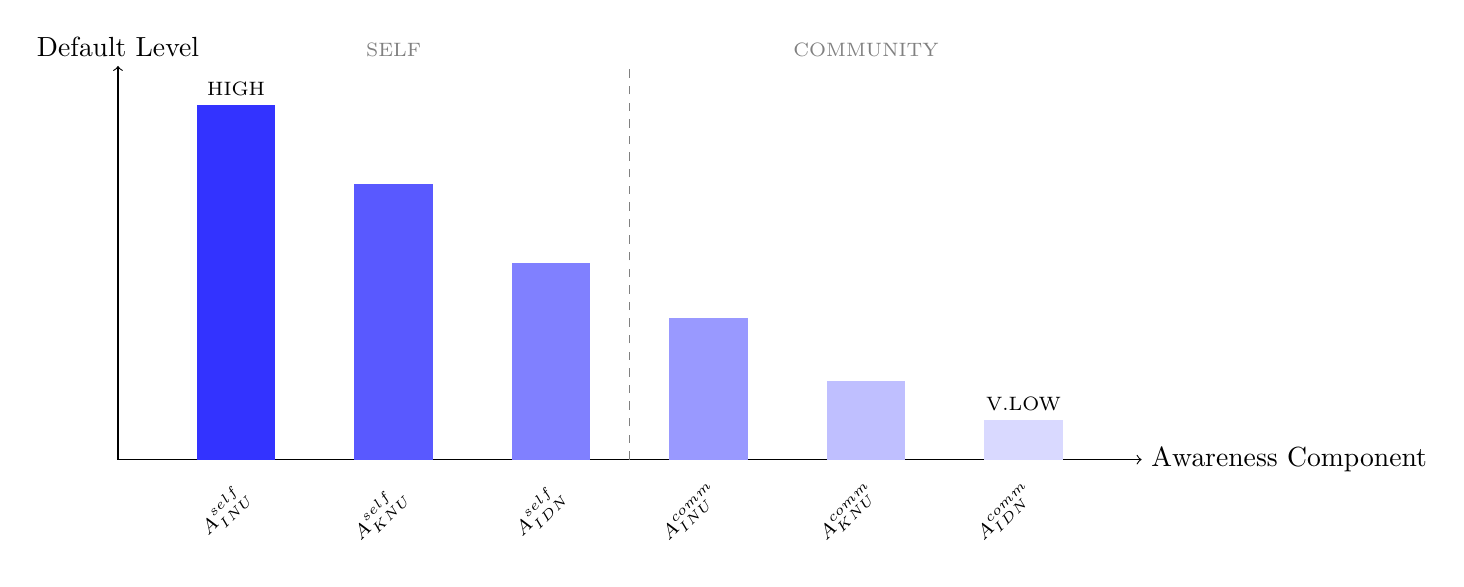
\begin{tikzpicture}
\draw[->] (0,0) -- (13,0) node[right] {Awareness Component};
\draw[->] (0,0) -- (0,5) node[above] {Default Level};

\fill[blue!80] (1,4.5) rectangle (2,0);
\fill[blue!65] (3,3.5) rectangle (4,0);
\fill[blue!50] (5,2.5) rectangle (6,0);
\fill[blue!40] (7,1.8) rectangle (8,0);
\fill[blue!25] (9,1.0) rectangle (10,0);
\fill[blue!15] (11,0.5) rectangle (12,0);

\node[below, font=\scriptsize, rotate=45, anchor=north east] at (1.5,-0.1) {$A^{self}_{INU}$};
\node[below, font=\scriptsize, rotate=45, anchor=north east] at (3.5,-0.1) {$A^{self}_{KNU}$};
\node[below, font=\scriptsize, rotate=45, anchor=north east] at (5.5,-0.1) {$A^{self}_{IDN}$};
\node[below, font=\scriptsize, rotate=45, anchor=north east] at (7.5,-0.1) {$A^{comm}_{INU}$};
\node[below, font=\scriptsize, rotate=45, anchor=north east] at (9.5,-0.1) {$A^{comm}_{KNU}$};
\node[below, font=\scriptsize, rotate=45, anchor=north east] at (11.5,-0.1) {$A^{comm}_{IDN}$};

\node[above, font=\scriptsize] at (1.5,4.5) {HIGH};
\node[above, font=\scriptsize] at (11.5,0.5) {V.LOW};

\draw[dashed, gray] (6.5,0) -- (6.5,5);
\node[above, font=\scriptsize, gray] at (3.5,5) {SELF};
\node[above, font=\scriptsize, gray] at (9.5,5) {COMMUNITY};
\end{tikzpicture}
\caption{The Awareness Gradient: Default Levels}
\label{fig:awareness-gradient}
\end{figure}

\paragraph{Why the Gradient Exists.}
The gradient reflects:
\begin{itemize}
\item \textbf{Evolutionary priority:} Self-preservation requires automatic self-awareness
\item \textbf{Cognitive cost:} Perspective-taking for others requires effort
\item \textbf{Information access:} Own states are directly felt; others' must be inferred
\item \textbf{Social distance:} Closer relationships activate more awareness
\end{itemize}

%------------------------------------------------------------------------------
\subsubsection{The Six Components in Detail}
%------------------------------------------------------------------------------

\paragraph{1. $A^{self}_{INU}$: Own Individual Utility Awareness.}
\begin{itemize}
\item \textbf{Content:} Personal gains and pains across FEPSDE dimensions
\item \textbf{Question:} ``What's in it for me?''
\item \textbf{Default level:} HIGH (self-interest is default)
\item \textbf{Activation:} Usually automatic, requires no effort
\item \textbf{Example:} ``This will cost me \euro{500}''
\end{itemize}

\paragraph{2. $A^{self}_{KNU}$: Own Collective Utility Awareness.}
\begin{itemize}
\item \textbf{Content:} Effects on groups the person belongs to
\item \textbf{Question:} ``How does this affect us/my people?''
\item \textbf{Default level:} MEDIUM (activated by group cues)
\item \textbf{Activation:} Requires group salience or social context
\item \textbf{Example:} ``This will help our team succeed''
\end{itemize}

\paragraph{3. $A^{self}_{IDN}$: Own Identity Utility Awareness.}
\begin{itemize}
\item \textbf{Content:} Identity confirmation or threat
\item \textbf{Question:} ``Is this consistent with who I am?''
\item \textbf{Default level:} LOW to MEDIUM (activated by value conflicts)
\item \textbf{Activation:} Triggered by identity-relevant situations
\item \textbf{Example:} ``A person like me would/wouldn't do this''
\end{itemize}

\paragraph{4. $A^{comm}_{INU}$: Community Individual Utility Awareness.}
\begin{itemize}
\item \textbf{Content:} Effects on others' personal welfare
\item \textbf{Question:} ``How does this affect them individually?''
\item \textbf{Default level:} LOW (requires perspective-taking)
\item \textbf{Activation:} Requires empathy or explicit prompting
\item \textbf{Example:} ``This will stress my employees''
\end{itemize}

\paragraph{5. $A^{comm}_{KNU}$: Community Collective Utility Awareness.}
\begin{itemize}
\item \textbf{Content:} Effects on others' groups
\item \textbf{Question:} ``How does this affect their communities?''
\item \textbf{Default level:} VERY LOW (requires extended perspective)
\item \textbf{Activation:} Requires deliberate, abstract thinking
\item \textbf{Example:} ``This affects their entire village''
\end{itemize}

\paragraph{6. $A^{comm}_{IDN}$: Community Identity Utility Awareness.}
\begin{itemize}
\item \textbf{Content:} Effects on others' identity
\item \textbf{Question:} ``How does this affect who they are?''
\item \textbf{Default level:} VERY LOW (requires deep empathy)
\item \textbf{Activation:} Requires sophisticated perspective-taking
\item \textbf{Example:} ``This threatens their professional identity''
\end{itemize}

%------------------------------------------------------------------------------
\subsubsection{Who Is the ``Relevant Community''?}
%------------------------------------------------------------------------------

The relevant community consists of \emph{other people whose utility the 
decision-maker considers}. This is context-dependent:

\begin{table}[htbp]
\centering
\caption{Types of Relevant Communities}
\label{tab:relevant-community}
\renewcommand{\arraystretch}{1.3}
\begin{tabular}{@{}llll@{}}
\toprule
\textbf{Scope} & \textbf{Examples} & \textbf{When Activated} & \textbf{$A^{comm}$ Level} \\
\midrule
Immediate & Family, close friends & Personal decisions & Higher \\
Proximate & Colleagues, neighbors & Work/local decisions & Medium \\
Extended & Organization, profession & Professional decisions & Lower \\
Abstract & Citizens, future generations & Policy, ethics & Very low \\
Global & Humanity, other species & Environmental, moral & Minimal \\
\bottomrule
\end{tabular}
\end{table}

\paragraph{The Identification Condition.}
For a community to be ``relevant,'' the decision-maker must:
\begin{enumerate}
\item \textbf{Identify} the community (know who they are)
\item \textbf{Consider} them (include in mental model)
\item \textbf{Care} about their utility (assign some weight)
\end{enumerate}

%------------------------------------------------------------------------------
\subsubsection{Implications of the Gradient}
%------------------------------------------------------------------------------

The awareness gradient explains systematic behavioral patterns:

\begin{table}[htbp]
\centering
\caption{Behavioral Implications of the Awareness Gradient}
\label{tab:gradient-implications}
\renewcommand{\arraystretch}{1.3}
\begin{tabular}{@{}ll@{}}
\toprule
\textbf{Observation} & \textbf{Awareness Explanation} \\
\midrule
Self-interest dominates & $A^{self}_{INU}$ highest by default \\
Collective action is hard & $A^{self/comm}_{KNU}$ requires activation \\
Distant others ignored & $A^{comm}$ requires deliberate effort \\
Abstract victims less compelling & $A^{comm}_{INU}$ for ``statistics'' very low \\
Identifiable victims more compelling & Specific person raises $A^{comm}_{INU}$ \\
Identity trumps interest & $A^{self}_{IDN}$ (when activated) can override $A^{self}_{INU}$ \\
\bottomrule
\end{tabular}
\end{table}

%------------------------------------------------------------------------------
\subsubsection{BEATRIX Module Reference}
%------------------------------------------------------------------------------

\begin{table}[htbp]
\centering

%------------------------------------------------------------------------------
\subsubsection{Time-Delayed Individual Utility: AWX-A1c}
%------------------------------------------------------------------------------

A critical extension of the two-level structure addresses \textbf{temporal delays}
in individual utility awareness:

\begin{axiom}[AWX-A1c: Zeitverzögerter INU]
Anticipation of delayed individual utility becomes salient only when the time 
horizon exceeds an instant threshold.

\textbf{Formal Condition:}
\begin{equation}
N_{ind}(t+h) \text{ salient} \Leftrightarrow h > \theta_{instant}
\end{equation}
where $\theta_{instant}$ is the threshold separating instant from delayed 
outcomes (typically seconds to minutes).
\end{axiom}

\paragraph{Implication.}
This axiom explains why:
\begin{itemize}
    \item Retirement savings (30-year horizon) require deliberate $A^{self}_{INU}$ activation
    \item Immediate consumption ($h < \theta_{instant}$) activates automatically via SYS 0
    \item Intermediate horizons (weeks to months) show variable awareness patterns
\end{itemize}

The interaction with AWX-A4 (Instant Exception) creates a discontinuity: 
outcomes below the threshold bypass the awareness requirement entirely, while 
outcomes above require the full awareness transformation chain.

\caption{Section 11.4 BEATRIX References}
\label{tab:11-4-beatrix}
\renewcommand{\arraystretch}{1.3}
\begin{tabular}{@{}lll@{}}
\toprule
\textbf{Element} & \textbf{Module} & \textbf{Reference} \\
\midrule
Self Utility & 7234\_INU, 7235\_KNU, 7236\_IDN & Utility categories \\
Community Relevance & AWX-A1a & Community-Relevanz \\
External Effects & AWX-A1b & Soziale Externeffekte \\
Awareness Differentiation & AWX-A34 & Category differences \\
\bottomrule
\end{tabular}
\end{table}

%%%%%%%%%%%%%%%%%%%%%%%%%%%%%%%%%%%%%%%%%%%%%%%%%%%%%%%%%%%%%%%%%%%%%%%%%%%%%%%
% END OF SECTION 11.4
%%%%%%%%%%%%%%%%%%%%%%%%%%%%%%%%%%%%%%%%%%%%%%%%%%%%%%%%%%%%%%%%%%%%%%%%%%%%%%%
